%!TEX root = foo-thesis.tex

\chapter{Preprocessing}
\label{chap:preproc}

Die Berechnung der Featurevektoren zur Schadenserkennung wird nicht unmittelbar auf der eingehenden Punktwolke ausgeführt, sondern bedarf zunächst einer Vorprozessierung. \\
Die erste Aufgabe besteht darin, den Boden der Punktwolke zu bestimmen und damit die Menge der für diesen Anwendungsfall überhaupt bedeutsamen Punkte zu reduzieren. Dazu wird eine Bodenerkennung (\textit{Ground Detection}) eingesetzt, welche unter anderem mit Höhenmodellen arbeitet und im Projekt auf der im \texttt{PCTool} bereits bestehenden Funktionalität aufbaut. Schließlich werden die als Boden erkannten Punkte mit der entsprechenden semantischen Klasse markiert. Der nachfolgende Schritt beruht auf einem guten Ergebnis der Bodenerkennung in dem Sinne, dass möglichst viele Punkte der Straße erhalten bleiben und restliche Punkte nicht die Bodenklasse zugewiesen bekommen. Auf die Hintergründe und Implementierung der ausgereifteren Bodenerkennung wird hier nicht näher eingegangen, dies ist bei \cite{Mattes-2021} zu finden.

\section{Straßenextraktion}

Mit den Informationen zum Boden folgt der Schritt, der die Straße selbst erkennen soll. Diese Straßenextraktion soll also außenstehenden Rasen, niedrige Häuserwände und sonstige als Boden klassifizierte, aber nicht zur Fahrbahn selbst gehörenden Bereiche entfernen. Die Grundlage dafür ist eine Abschätzung der Trajektorie des \textit{Mobile-Mapping}-Fahrzeugs, also dessen gefahrener Strecke, die ja auf der Straße verläuft. Diese Abschätzung beruht auf den Dichten der einzelnen Punkte, das bedeutet wie viele Nachbarn sie in einem gewissen Radius besitzen. Bedingt durch die Arbeitsweise der Laserscanner werden nämlich nahegelegene Oberflächen deutlich dichter abgetastet als weiter entfernte \citep{Li.etal-2019}. Wegen der Montierung des Laserscanners auf dem Fahrzeug sind die Punkte auf der gefahrenen Strecke entsprechend dichter als etwa die andere Straßenseite und sonstige Oberflächen. Eine Visualisierung dessen findet sich in Abbildung \ref{fig:colored_density}. \\

\begin{figure}
    \subcaptionbox{Die Straße eingefärbt nach dem Intensitätswert.}{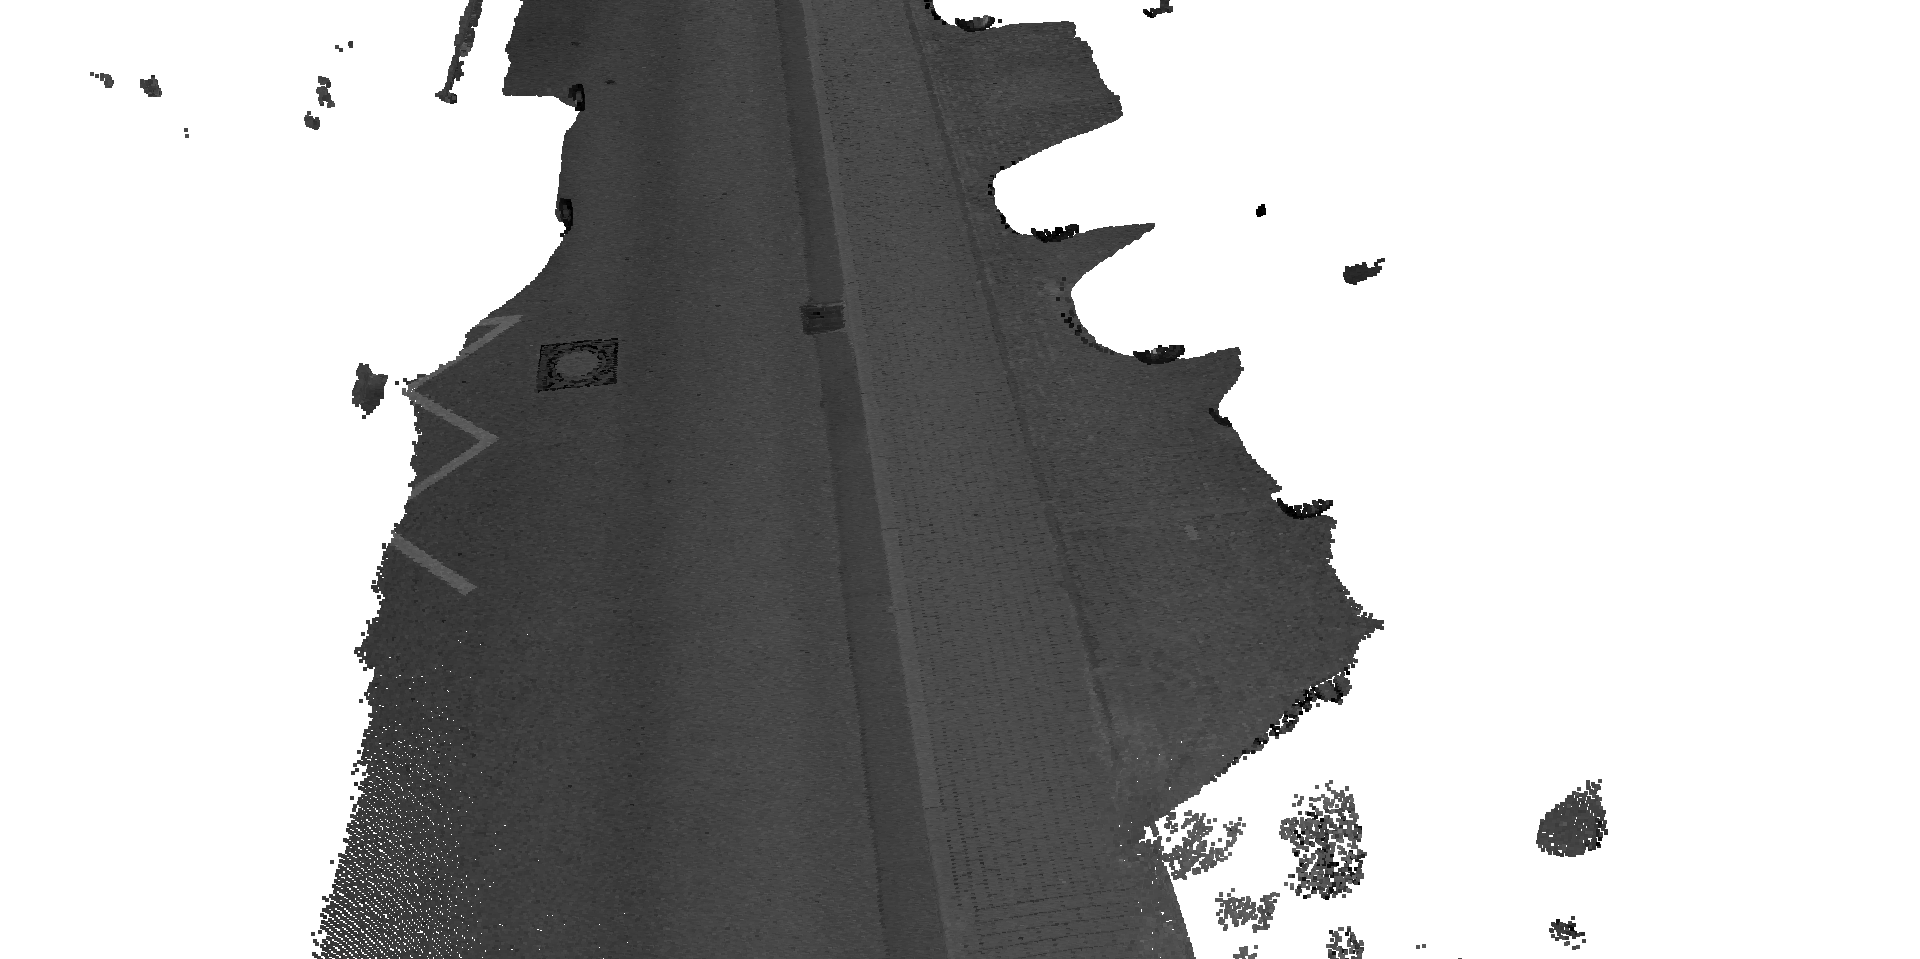
\includegraphics[width=0.5\textwidth]{graphics/trajectory_intensity}}
    \hfill
    \subcaptionbox{Die Straße eingefärbt nach ihren Punktdichten.}{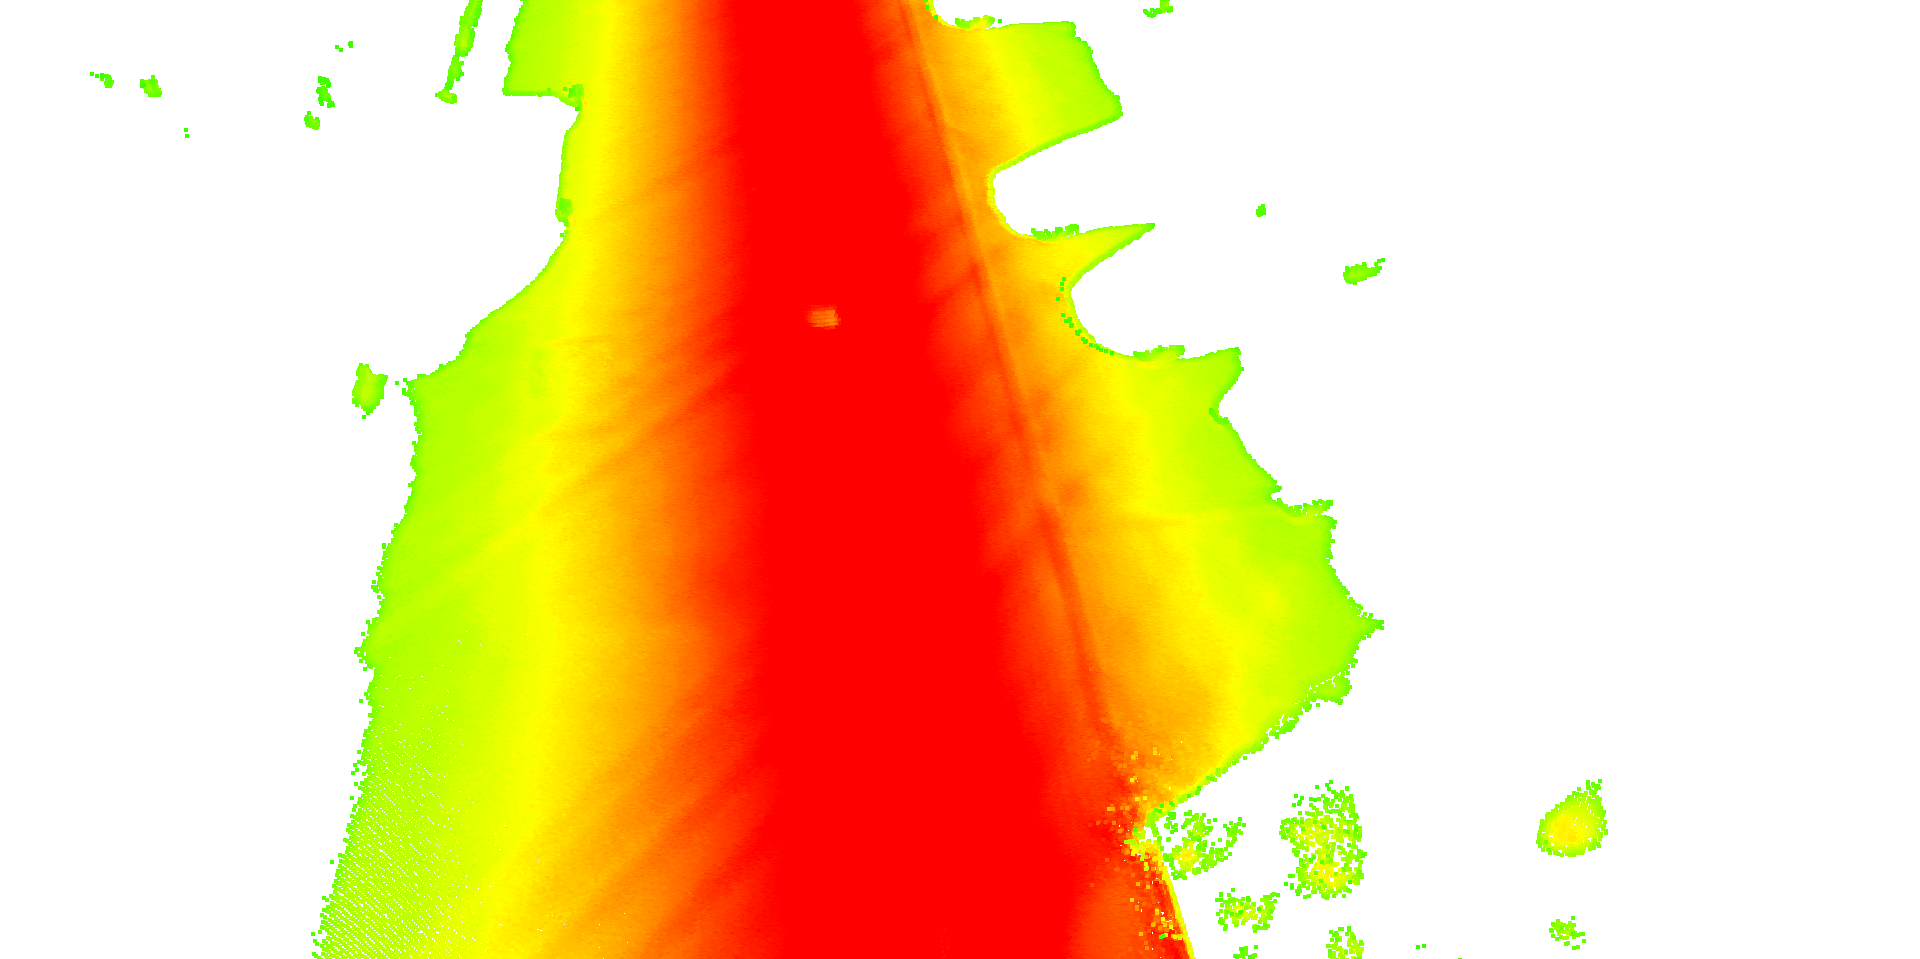
\includegraphics[width=0.5\textwidth]{graphics/trajectory_colored}}
    \caption{Eingefärbte Dichten der Punktwolke nach stattgefundener Bodenerkennung und Entfernung des Nicht-Bodens. Je roter der Farbton eines Punktes, umso dichter ist dessen Umgebung. Die abgeschätzte Trajektorie umfasst eine Straßenseite sowie den Gehweg auf dieser Seite.}
    \label{fig:colored_density}
\end{figure}

Da sich die konkreten Dichten je nach genutztem Laserscanner und somit pro Punktwolke unterscheiden können, werden die gesammelten Dichten zu relativen Werten umgewandelt. Dabei kommt die sogenannte \textit{Min-Max}-Normalisierung zum Einsatz \citep{Patro.Sahu-2015}. Das bedeutet, von jedem einzelnen Wert der Liste - hier der Dichten pro Punkt - wird das Minimum der Liste subtrahiert und anschließend durch die Differenz von Maximum und Minimum geteilt. Auf diese Weise ist in der verarbeiteten Liste immer der kleinste Wert die 0 und der größte Wert die 1. Diese nun relativen Dichten sind über verschiedene Punktwolken hinweg besser vergleichbar. \\\\
Mit Hilfe des arithmetischen Mittels und der Standardabweichung der relativen Dichten wird die Punktwolke in zwei Teile getrennt: Der erste Teil repräsentiert die abgeschätzte Trajektorie, die zumindest größtenteils zur Straße dazugehören soll. Der zweite Teil beinhaltet die restlichen Punkte, wozu die andere Straßenseite und sonstige übrig gebliebene Oberflächen zählen können, die also teilweise auch als Straße erkannt werden sollen. Dabei zählen all jene Punkte, deren relative Dichte größer als das arithmetische Mittel minus einer halben Standardabweichung ist, zum Trajektorie-Teil. Der Faktor wurde empirisch bestimmt. \\
Auf den beiden Teilen wird nun parallel der \texttt{PointCloudClusterer} eingesetzt, der bereits im \texttt{PCTool} integriert ist: Dieser ermittelt auf Punktdistanzen basierende zusammenhängende Bereiche, die \textit{Cluster}. Spezifiziert werden kann die maximale Distanz eines Punktes zur Noch-Zugehörigkeit zu einem \textit{Cluster} sowie die minimale Größe eines \textit{Clusters} gegen sein Verwerfen. 
Die maximale Distanz wurde hier auf 20\% der durchschnittlichen relativen Dichte gesetzt, was bei den getesteten Punktwolken einen guten Ausgleich zwischen Straßenbeibehaltung und Entfernung restlicher Punkte bedeutete. Die nötige Größe der \textit{Cluster} beträgt 30\% der Größe der jeweiligen Teilpunktwolke. Dies beruht auf der Annahme, dass in beiden Teilen die Straße den jeweils größten Anteil der Punkte ausmacht, da sie durchgängig verläuft im Gegensatz zu Rasenflächen einzelner Gebäude oder sonstigen nahegelegenen Bodenstellen. Andererseits wird nicht zwangsläufig nur das größte \textit{Cluster} behalten, da es Fälle geben kann, in denen die Straße getrennt voneinander ist - etwa durch parkende Autos, die durch die vorherige Bodenerkennung entfernt worden sind. Diese 30\% sollen also erneut einen Ausgleich herstellen zwischen einer vollständigen Straßenerfassung und möglichst großen Entfernung sonstiger Punkte. All jene \textit{Cluster}, die bis dahin übrig geblieben sind - im Trajektorie-Teil wie im restlichen Teil - werden zur Straße gezählt und zum Schluss wieder zu einer einzelnen Punktwolke zusammengeführt mit dem integrierten \texttt{PointCloudMerger}. Eine geordnete Darstellung dieses Prozesses findet sich in Abbildung \ref{fig:street_extraction}.

\begin{figure}[!ht]
    \centering
    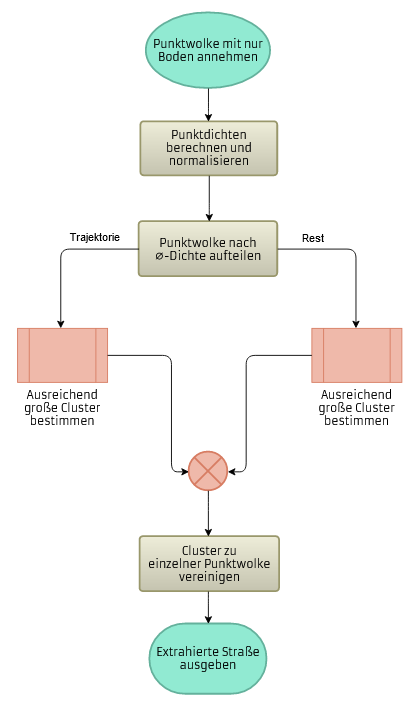
\includegraphics[width=0.5\textwidth]{graphics/flowchart_street_extraction}
    \caption{Eine Übersicht des Ablaufs der Straßenextraktion. Die roten Kästen kennzeichnen die bezüglich Laufzeit aufwändigsten Schritte des Prozesses.}
    \label{fig:street_extraction}
\end{figure}

Dieser Teil der gesamten \textit{Pipeline} sollte keinen Fokus der Arbeit einnehmen, sondern war zunächst rein funktional angelegt und beruht auf einigen Heuristiken. Wie in Kapitel \ref{chap:eval} dargestellt wird, reicht dies bereits aus für den Erhalt der fast vollständigen Straße und großer Reduktion sonstiger Punkte. Nachteilig ist, dass der Prozess Parameter beinhaltet, die bisher nur nach reinem Empfinden und an wenigen Testpunktwolken bestimmt wurden. Für denkbare Verbesserungen der Straßenextraktion neben diesem Ansatz siehe Kapitel \ref{chap:outro}. \\
Sobald die nun als Straße erkannten Punkte extrahiert sind, dient die nun übrige Punktwolke beiden Ansätzen als Eingabe ihrer Verarbeitung.

\section{Normalisierung der Intensität}

Vor der tatsächlichen Berechnung der Features erfolgt noch eine Wertenormalisierung. Während der \textit{Deep-Learning}-Ansatz seine eigene Art der Normalisierung vornimmt, geht der eigene Ansatz folgendermaßen vor: 
Oftmals wird neben den 3D-Koordinaten der Punkte auch ihre Intensität erfasst und gespeichert, ein Maß zur Ermittlung der Stärke des reflektierten Laserstrahls \citep{Tatoglu.Pochiraju-2012}. Dieses Intensitätsattribut besitzt eine hohe Varianz bezüglich verschiedener Laserscanner, die unter anderem von deren unterschiedlicher Technik oder Verarbeitung verursacht wird. Zwar liegt der Wertebereich des Attributs grundsätzlich bei 0 bis 65535, wird aber meist nicht ausgenutzt. Der Intensitätswert desselben Punktes, aufgenommen von zwei verschiedenen Laserscannern, kann sich um mehrere Tausend unterscheiden. Aus diesem Grund werden diese absoluten Werte zunächst in relative umgewandelt, sodass sie über verschiedene Punktwolken hinweg vergleichbar sind. Für die Normalisierung wird ebenfalls die \textit{Min-Max}-Normalisierung verwendet, wie sie im vorigen Abschnitt erläutert wurde. Dadurch hat letztlich die geringste Intensität der Punktwolke den Wert 0 und die höchste den Wert 1. Eine ähnliche Normalisierung und Anpassung des Wertebereichs findet sich bei \cite{Li.Cheng-2018}. Ein Nachteil dessen ist der Verlust der absoluten Dimension der Intensität. Dies könnte zum Beispiel dann problematisch sein, wenn eine Punktwolke keine Fahrbahnmarkierungen beinhaltet, die für gewöhnlich die hellsten Objekte auf der Straße sind. In diesem Fall würden durch die Normalisierung Punkte einer anderen Klasse die höchsten Werte nahe der 1 erhalten, was sich unter Umständen negativ auf die auf diesem Feature aufbauenden \textit{Predictions} auswirkt. \\
Da bei den 3D-Koordinaten keine so erheblichen Unterschiede zu erwarten sind, werden diese Werte nicht normalisiert und alle letztlich daraus ermittelten Features als vergleichbar über verschiedene Punktwolken hinweg angesehen. \\\\
Ein weiterer Aspekt, der eine schädliche Wirkung auf die Qualität der \textit{Predictions} haben kann, sind einzelne Punkte, deren Intensität übermäßig stark von der Mehrheit der anderen Werte abweicht. Unabhängig davon, ob dies Messungenauigkeiten sind oder tatsächlich einzelne Abweichungen, wird diese Anomalie in die Normalisierung übernommen und daher ist ein Entfernen jener Werte erstrebenswert. Da aber selbstverständlich auch diese Punkte erhalten bleiben und eine Intensität besitzen sollen, werden die Außenseiter-Punkte noch vor der Normalisierung bestimmt und ihre Intensität auf den niedrigsten bzw. höchsten Wert gesetzt, der nicht zu den abweichenden Werten gezählt wird. Auf diese Weise sollen die Relationen zwischen verschiedenen Punktwolken annähernd erhalten bleiben, ohne durch die Werteanpassung und anschließende Normalisierung einen merklichen Informationsverlust zu erleiden. \\
Der hier genutzte Prozess zum Finden abweichender Punkte basiert auf der \textit{Interquartile Range (IQR)} \citep{Rousseeuw.Hubert-2011}. Dabei werden die Werte an einem Viertel sowie drei Viertel (zur Ganzzahl abgerundet bzw. aufgerundet) der sortierten Liste angeschaut: Dies sind das erste bzw. dritte Quartil $Q_1, Q_3$. Mittels $IQR = Q_3 - Q_1$ können nun die angesprochenen Schwellwerte nach oben und nach unten definiert werden als
\begin{equation}
    T_{lo} = Q_1 - s * IQR  
        \quad\text{und}\quad 
    T_{hi} = Q_3 + t * IQR
\end{equation}
Alle Werte kleiner als $T_{lo}$ werden schließlich auf $T_{lo}$ gesetzt; alle Werte größer als $T_{hi}$ werden auf $T_{hi}$ gesetzt. Die einzigen Parameter, die dafür noch festgelegt werden müssen, sind $s$ und $t$. Sie bestimmen, wie schnell ein Wert als Außenseiter betrachtet wird. Häufig liegen um $1,5$, in diesem Fall werden sie - auch bedingt durch die große Spannbreite des Wertebereichs mit starker Konzentration in der Mitte wegen der gewöhnlichen Straßenpunkte - empirisch mit $s=6$ bzw. $t=4$ belegt. Konkrete Zahlen zu den Auswirkungen auf Trainings- und Testpunktwolke finden sich in Kapitel \ref{chap:eval}.